\documentclass[12pt]{article}
\usepackage{makeidx}
\usepackage{multirow}
\usepackage{multicol}
\usepackage[dvipsnames,svgnames,table]{xcolor}
\usepackage{graphicx}
\usepackage{epstopdf}
\usepackage{ulem}
\usepackage{hyperref}
\usepackage{amsmath}
\usepackage{amssymb}
\author{}
\title{CNTAC 2024A}
\usepackage[paperwidth=600pt,paperheight=780pt,top=38pt,right=40pt,bottom=40pt,left=40pt]{geometry}

\newcommand{\ha}{H$\alpha$}
\newcommand{\Msun}{\mathrm{M}_\odot}

\begin{document}

{\raggedright

\vspace{3pt} \noindent
\begin{tabular}{|p{514pt}|}
\hline
\parbox{514pt} {\raggedright \vspace{3pt} The maximum length of this
  file is \textbf{5 pages TOTAL} (7 for long-term + large programs)
  and it must include the following aspects: Anonymous scientific aim and
  rationale (3-page limit), anonymous technical
  description (1-page limit), anonymous justification for long-term status if
  applicable (1-page limit), non-anonymous work plan for large-programs (1-page
  limit), non-anonymous description of the current status of the project including
  publications and student thesis context if applicable(1-page limit). All these limits include table, figures, captions, references, etc. for each section. \textbf{This template must not be edited. This means no
    alteration of font size of main texts or margins. Please DO REMOVE
    this paragraph as it is intended as information only. }} \\ \hline
\end{tabular}
\vspace{2pt}
}

\texttt{\textbf{SCIENTIFIC AIM AND RATIONALE} \\ }

% Example clusters for figure: 
% name                     ra         dec      SNR
% ACT-CL J0125.0-0531   21.271394 	-5.517004   11.1
% ACT-CL J0156.3-0123   29.098821 	-1.384531   8.3
% ACT-CL J0355.9-3741   58.993665 	-37.693496 	9.2 very rich on 10' scale
% ACT-CL J0509.3-5342 	77.336482 	-53.703352 	14.8  strong lensing
% ACT-CL J0826.0+0419 	126.517953 	4.324603 	13.7
% ACT-CL J0929.9+1520 	142.493189 	15.341605 	5.7 very loose
% ACT-CL J1047.4-0104 	161.853632 	-1.070364 	10.0 merger? two bcgs
% ACT-CL J1156.0+0529 	179.020045 	5.484386 	7.5  merger? two bcgs
% ACT-CL J1256.2+1635 	194.051460 	16.588171 	5.9 strong lensing
% ACT-CL J1305.7+1417 	196.448392 	14.294955 	4.6 lonely BCG - fossil?
% ACT-CL J2145.8-5645 	326.469875 	-56.750497 	16.3 faint giant SL arcs
% ACT-CL J2342.2+1315 	355.554232 	13.262693 	4.8 giant arc?

% from 10' images:
% ACT-CL J0355.9-3741
% ACT-CL J0841.3+1141
% ACT-CL J1156.0+0529
% ACT-CL J1513.7+0525

The evolution of a galaxy is deeply connected to its environment. While galaxies living in low-density environments, such as the Milky Way, are usually star-forming spirals, those in high-density environments are by and large passively evolving elliptical galaxies with little or no star formation.

While this picture captures well the overall interaction between a galaxy's evolutionary stage and its environment, in detail there are many open questions. It has been found, for instance, 



\begin{figure}
\centering
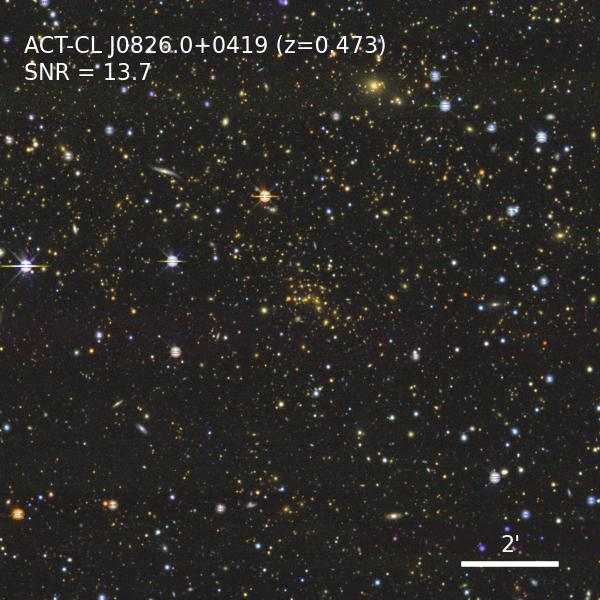
\includegraphics[width=0.49\linewidth]{plots/ACT-CL_J0826.0+0419__20_0.262.jpg}
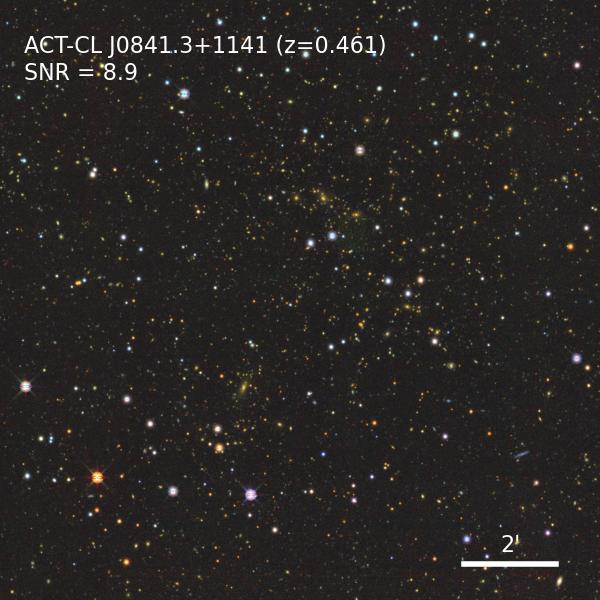
\includegraphics[width=0.49\linewidth]{plots/ACT-CL_J0841.3+1141__20_0.262_altcen.jpg}
\caption{Optical images of two example clusters, highlighting the diversity of systems we propose to observe. Images are centered around the galaxy distribution rather than the SZ signal. \textbf{Other groupings near J0841 are not detected in SZ (2018d maps); what about photo-z?}}
\label{f:imgs}
\end{figure}



\clearpage
\texttt{\textbf{TECHNICAL DESCRIPTION} \\ }

We will follow Khostovan et al.\ (2020) in the reduction and line measurements, including contamination corrections.

The DECam field-of-view covers each cluster in its entirety, out to at least $2r_{200}$, where $r_{200}$ is the radius enclosing 200 times the critical density. This will allow us to measure \ha\ profi

\textbf{Radially-binned Ha luminosity function/SFR}

We propose to observe XX SZ-selected clusters with \textit{spectroscopic redshifts} in the range $0.46\leq z\leq0.48$, where the H$\alpha$ line falls within the FWHM of the NB964 filter. 

We set the required exposure time to achieve a specific star formation rate (sSFR) limit of $10^{-11}\,\mathrm{yr^{-1}}$, i.e., the typical limit used to differentiate passive and star-forming galaxies (e.g., XXXX), which for a typical galaxy of $M_\star=10^{10}\,\Msun$ corresponds to a SFR of $\dot M_\star = 0.1\,\Msun\,\mathrm{yr^{-1}}$. Using the Kennicutt (1998) law as a benchmark and accounting for the typical contamination of the H$\alpha$ flux by the $[N\textsc{ii}]$ emission line in the NB964 filter (Khostovan et al.\ 2020) requires an H$\alpha$ luminosity of $9.3\times10^{39}\,\mathrm{erg\,s^{-1}}$, i.e., a flux of $4.9\times10^{-17}\,\mathrm{erg\,s^{-1}\,cm^{-2}}$. We scale the exposure time and limiting flux obtained in the NB964 survey of the COSMOS field by Khostovan et al.\ (2020), namely a 5$\sigma$ limit of $8.2\times10^{18}\,\mathrm{erg\,cm^{-2}s^{-1}}$ with an exposure of 47.25 hr. The requested exposure time per cluster is therefore 90 minutes. Assuming typical exposures of 600 s to avoid severely saturated stars, the dominant read-out overhead is $<5\%$; we conservatively assume a 10\% overhead and therefore request total observing time of 100 min per cluster, i.e., $28\times100\approx47$ hr. Typical slew angles of 50 deg result in 2 min slew overhead for a total of one hour slew overhead. \textbf{We therefore request a total of 48 hr of observing time}. We anticipate requesting the same observing time for semester 2024B.

Our target list spans the entire RA range; we will select the final targets from the uploaded target list depending on when the observing runs are scheduled if this proposal is approved.

\clearpage
\texttt{\textbf{JUSTIFICATION OF LONG-TERM STATUS OR WORK PLAN FOR LARGE PROGRAMS (IF APPLICABLE). \textbf{This paragraph can be deleted if it is not applicable to the proposal}} \\ }

\clearpage
\texttt{\textbf{CURRENT STATUS OF THE PROJECT} \\ }

% \texttt{\textbf{STUDENT THESIS}}
% if the data requested is identified as critical for
% a graduate student's thesis at a Chilean institution, explain the relevance of the data
% within the thesis and include the expected date of thesis defense \textbf{This paragraph can be deleted if it is not applicable to the proposal} \\



\end{document}
